%%%%%%%%%%%%%%%%%%%%%%%%%%%%%%%%%%%%%%%%%%%%%%%%%%%%%%%%%%%%%%%%%%%%%%%%%%%%%%%%%%%%%%%%%%
\section{Results and Discussion}


\subsection{Gradient decent methods}

\subsection{Neural Network}

\subsection{Classification}


%  ____            _         _ 
% |  _ \ __ _ _ __| |_    __| |
% | |_) / _` | '__| __|  / _` |
% |  __/ (_| | |  | |_  | (_| |
% |_|   \__,_|_|   \__|  \__,_|
%                              

%%%%%%%%%%%%%%% Run 1 %%%%%%%%%%%%%%%
% Line plot with varying number of mini-batches

In figure \ref{fig:d_line_batch_size} the Accuracy score is plotted for
different number of mini-batches. We observe that the convergence rate
increases with increasing number of mini-batches. This trend is expected. The
total amount of iterations/training is higher for a larger number for
mini batches. Another reason is that we are less likely to get stuck in global
minima, since the multiple different samples is used to calculate gradient of the
cost function. We also observe that the accuracy score tend to increase both
for the training and test data with increasing number of mini-batches.
We chose 20 number of mini-batches as our best value in the next. However, 15
number of mini-batches seems to give similar performance.    


\begin{figure}[H]
    \centering
    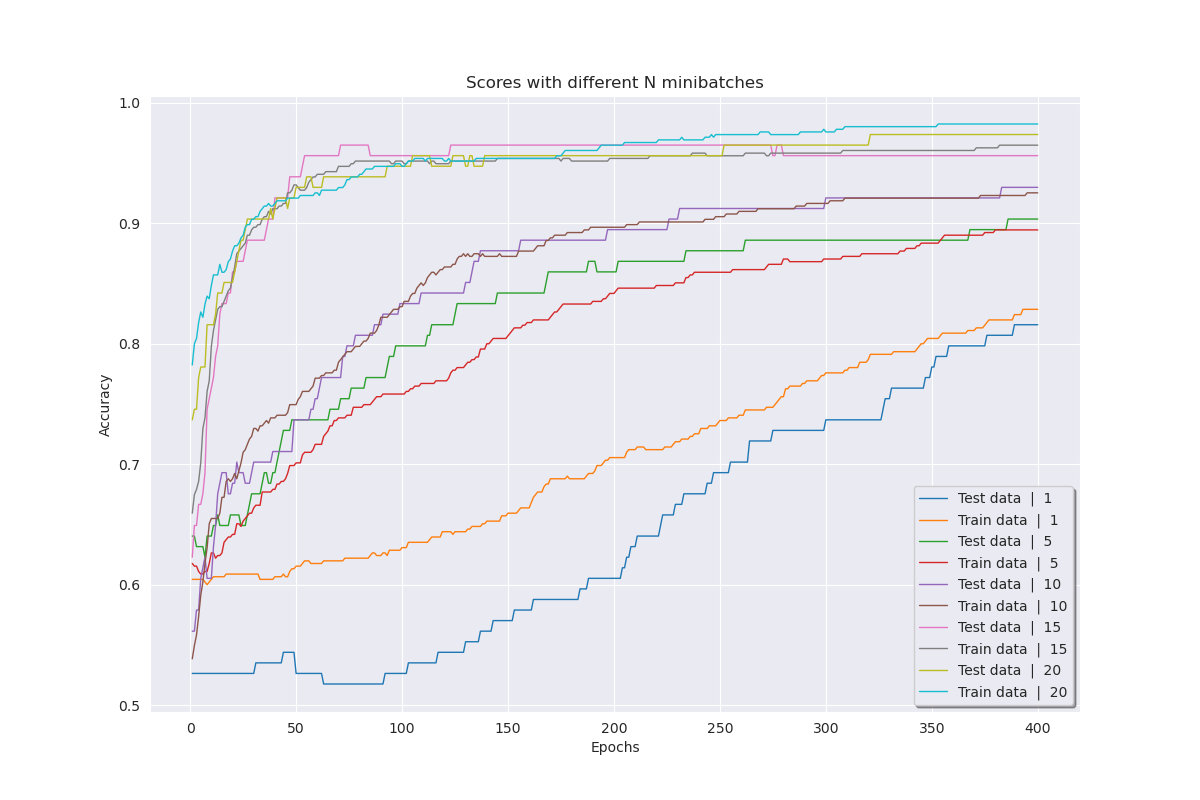
\includegraphics[width=0.8\textwidth]{Figures/PartD/d_line_batch_size.png}
    \caption{Accuracy score for train and test data plottet with respect to epochs for Run 1 (see table
    \ref{tab:runs_classification_cancer}). The number on the labels correspond
to number of mini-batches.}  
    \label{fig:d_line_batch_size} 
\end{figure}


%%%%%%%%%%%%%%% Run 2 %%%%%%%%%%%%%%%
% Lambda vs eta

In figure % XXX: ref

In figure \ref{fig:d_heatmap_train_eta_vs_lambda} and
\ref{fig:d_heatmap_train_eta_vs_lambda} is accuracy score for run 2 plotted for
different values of regularization parameter and learning rate for the training
and test data respectively. For our test data the best Accuracy of 0.9825 was
gotten with $\lambda = 10^{-4}$, $\eta = 0.1$ and $\lambda = 0.01$, $\eta =
0.01$. Generally we observe that the accuracy tend to increase with increasing
learning rate. This make sense since the model is learning faster. High
learning rates often leads exploding loss scores. This is not observed in this
case. By choosing the largest learning rate, we can maximize the accuracy and
minimize CPU cycles. 

We observe an increasing trend in accuracy with respect to increasing $\lambda $
values (Lambda in figure). This is more significant for the smaller values
of learning rate. To further study this trend we plotted the accuracy score
for different $\lambda $ values with respect to epochs in figure
\ref{fig:_d_line_different_lambdas}. We clearly see in increased convergence
rate for higher values of lambda. Moreover, the accuracy both for the train and
test data is higher for larger values of $\lambda $. For further fine-tuning of
parameters we will set $\lambda = 0$, to better observe how the different
parameters affect the score with respect to epochs. 


% FIXME: fix figures, 

\begin{figure}[H]
    \centering
    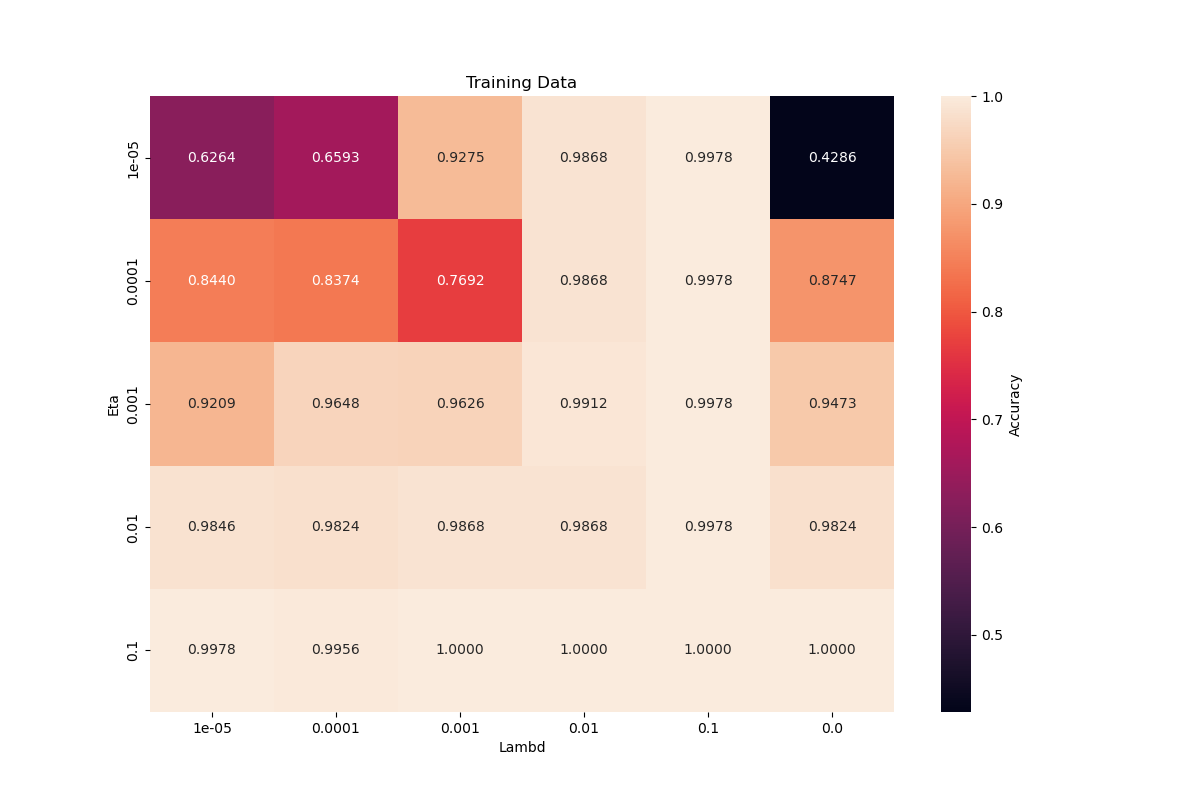
\includegraphics[width=\textwidth]{Figures/PartD/d_heatmap_train_eta_vs_lambda}
    \caption{Heatmap of accuracy score for training dta after 200 epochs with
    respect to different learning rates (Eta) and different L2-regularzation
    parameters (Lambd).   Spesific parameters used in run 2 is listed in table
\ref{tab:runs_classification_cancer}   }  
    \label{fig:d_heatmap_train_eta_vs_lambda}  
\end{figure}

\begin{figure}[H]
    \centering
    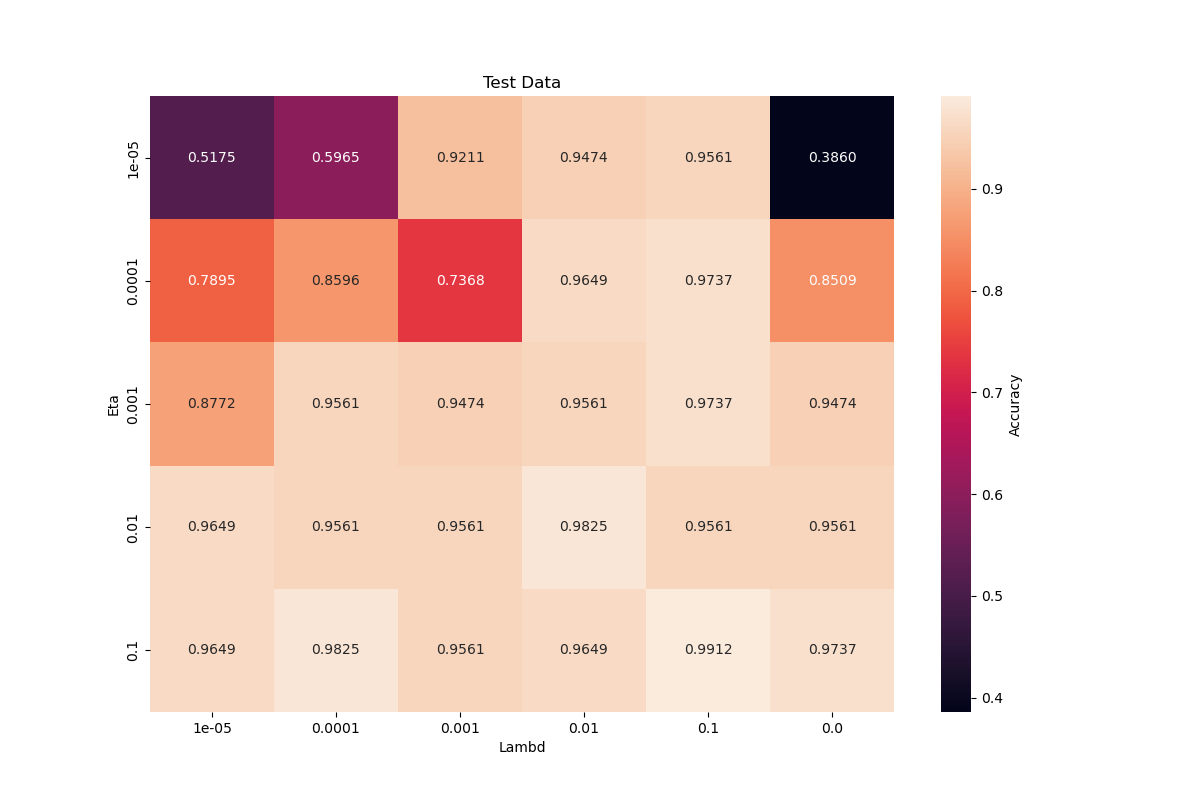
\includegraphics[width=\textwidth]{Figures/PartD/d_heatmap_test_eta_vs_lambda}
    \caption{Heatmap of accuracy score for test dta after 200 epochs with
    respect to different learning rates (Eta) and differn L2-regularization
    parameters (Lambda). Specific parameters used in run 2 is listed in table
    \ref{tab:runs_classification_cancer}       }  
    \label{fig:d_heatmap_test_eta_vs_lambda}  
\end{figure}


            
\begin{figure}[H]
    \centering
    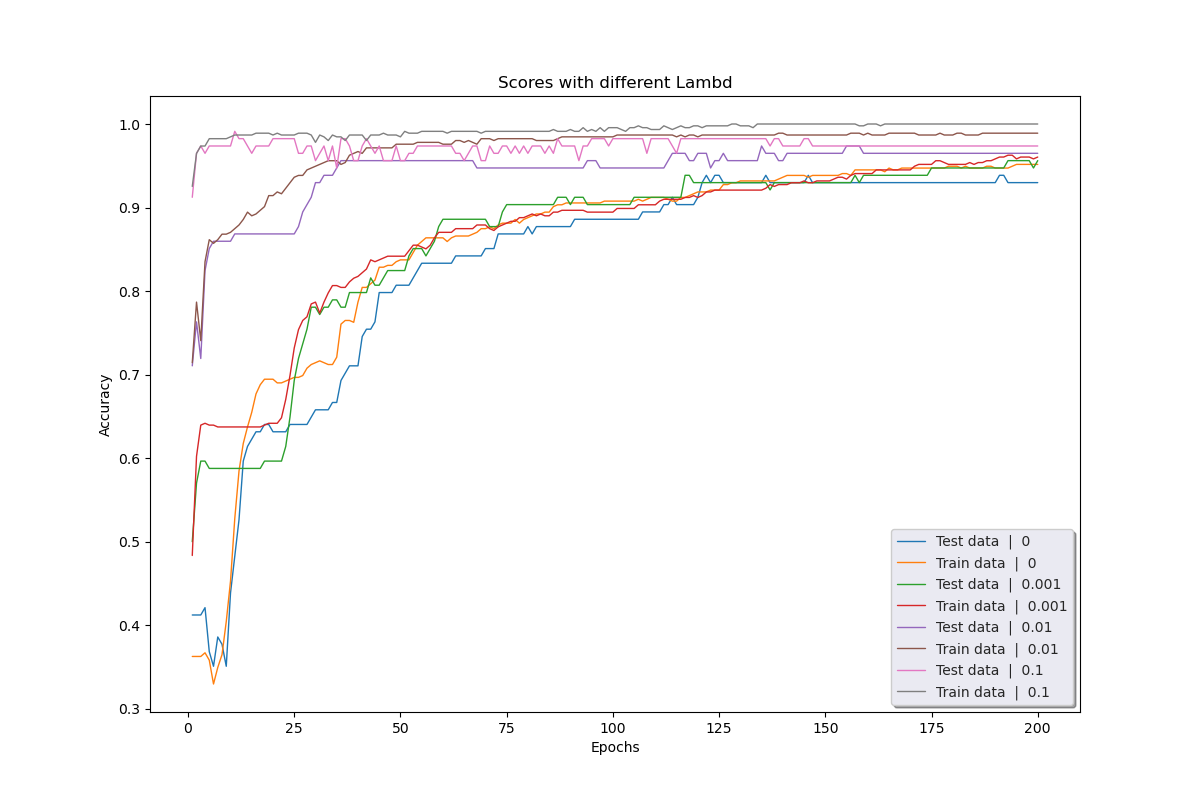
\includegraphics[width=0.8\textwidth]{Figures/PartD/_d_line_different_lambdas.png}
    \caption{Plot of accuracy score for training and test data with respect to
    epochs. Each line correspond to different values of $\lambda $ as indicated
by the number in the legend. A learning rate of 0.001 was used.}  
\label{fig:_d_line_different_lambdas} 
\end{figure}


%%%%%%%%%%%%%%% Run 3 %%%%%%%%%%%%%%%
% Depth vs width


In Run 3 different network architecture was tested with respect number of nodes
(width) and number of hidden layers (depth). The heat map's for the train and test
data is shown in figure \ref{fig:d_heatmap_train_depth_vs_width_lambd_0} and
\ref{fig:_d_heatmap_test_depth_vs_width_lambd_0}. For our test data the best
accuracy score was gotten with 2 hidden layers with 5 nodes in each, with an
accuracy of 0.9912. There is no clear trend with respect to architecture. We
will chose 2 hidden layers and 5 hidden nodes as our best parameters. However
the variations with respect to depth and width, may bet attributed to other random
phenomena such as mini-batch selection. There is no reason to chose a more
complex model since this will increase the computational cost of the network.      

% FIXME: not discussed training data


\begin{figure}[H]
    \centering
    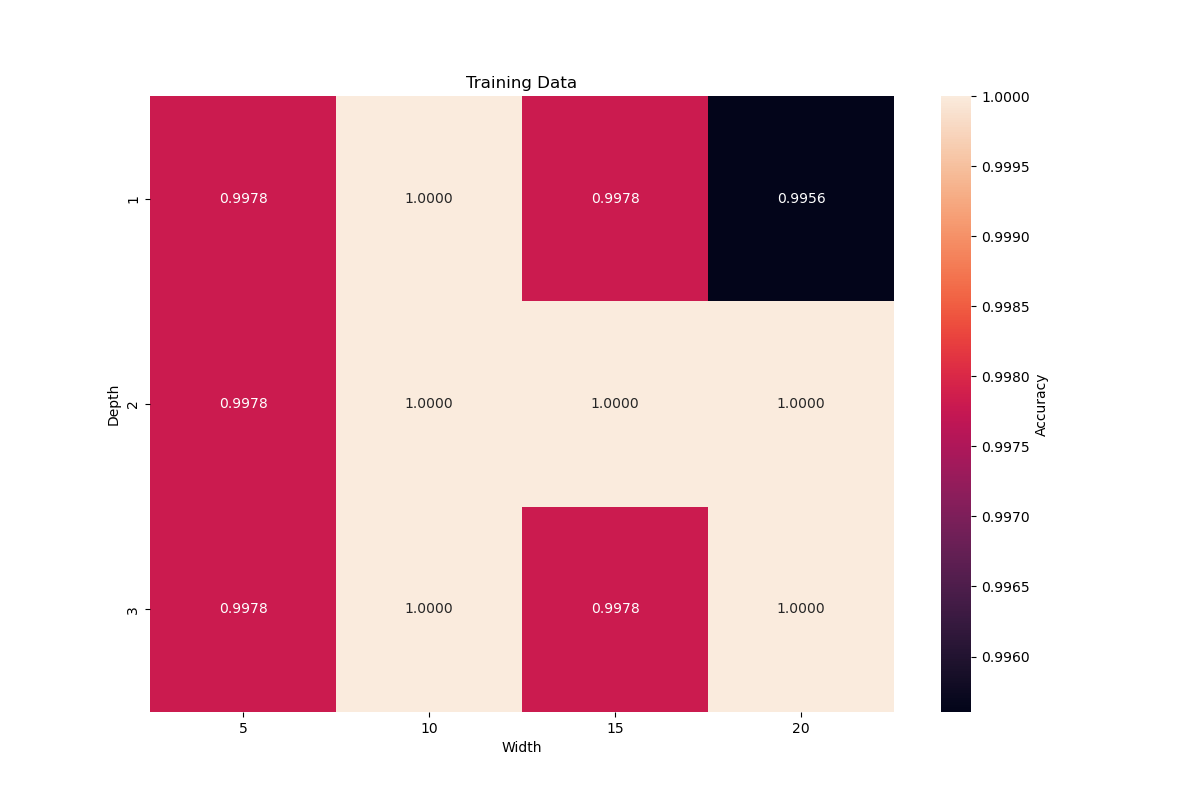
\includegraphics[width=0.8\textwidth]{Figures/PartD/d_heatmap_train_depth_vs_width_lambd_0.png}
    \caption{Accuracy score for train data with respect to different N number
        of hidden layers (depth) and number of hidden nodes in each hidden layer
    (width)  }  
    \label{fig:d_heatmap_train_depth_vs_width_lambd_0} 
\end{figure}


\begin{figure}[H]
    \centering
    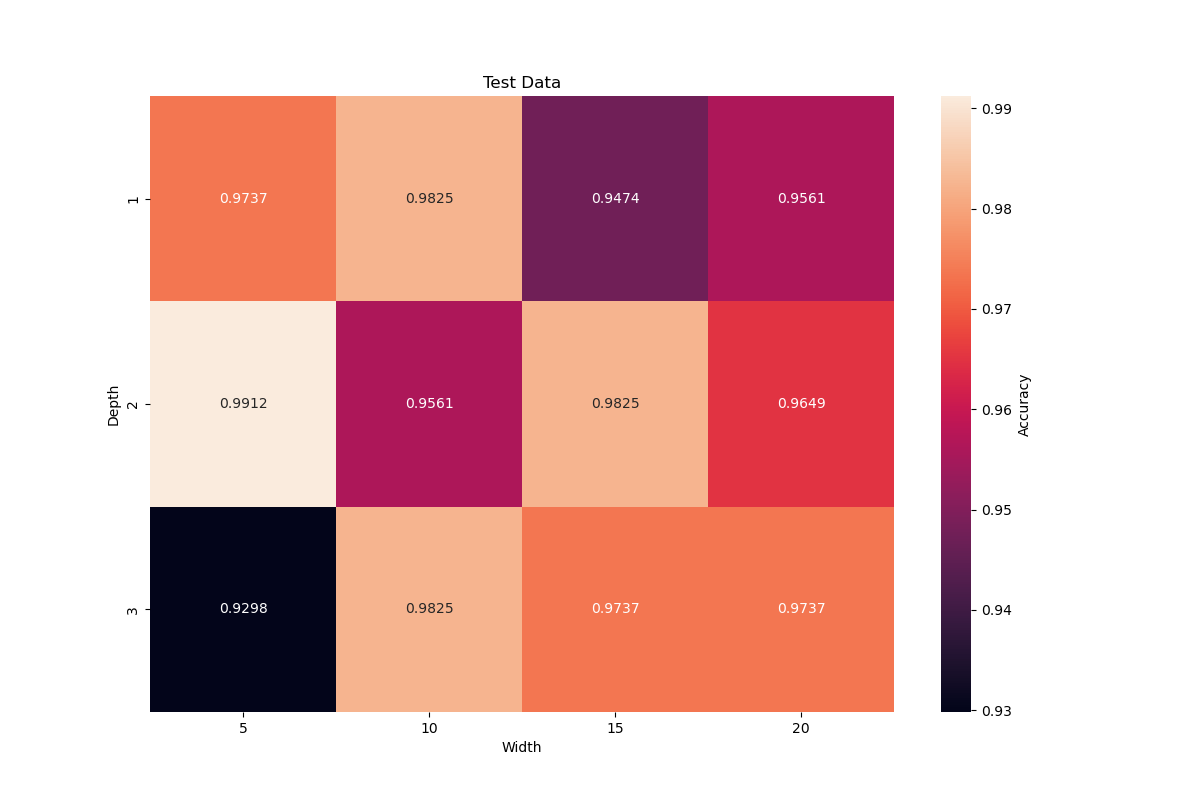
\includegraphics[width=0.8\textwidth]{Figures/PartD/_d_heatmap_test_depth_vs_width_lambd_0.png}
    \caption{Accuracy score for test data with respect to different N number
        of hidden layers (depth) and number of hidden nodes in each hidden layer
    (width)  }  
    \label{fig:_d_heatmap_test_depth_vs_width_lambd_0} 
\end{figure}

%%%%%%%%%%%%%%% Run 4 %%%%%%%%%%%%%%%
% Testing tuning method width and without momentum  

In Run 4 we tested different learning rate tuning methods. In figure
\ref{d_tuning_eta_0_001_with_gamma_0} the accuracy score is plotted
with respect to epochs for manual (none), adagrad, adman and the rms prop
tuning method. The learning rate parameter was set to 0.001. We observe that
RMS Prop and ADAM converges much faster than Adagrad and without any tuning.
The poor performance of Adgrad is probably due the low value initial value for
$\eta $. Both ADAM and RMS-prop performance well on both the training and test
data with a high accuracy and convergence after around 50 epochs. 

In figure \ref{fig:d_tuning_eta_0_001_with_gamma_0_9} the same lines are
plotted but with momentum, $\gamma = 0.9$. This causes a significant
improvement both the accuracy and convergence rate with Adagrad and plain SGD.   
Adagrad gives better prediction on the test data than both RMS prop and ADAM.
The added momentum to ADAM causes more fluctuations with respect to epochs than
without momentum.  

\begin{figure}[H]
    \centering
    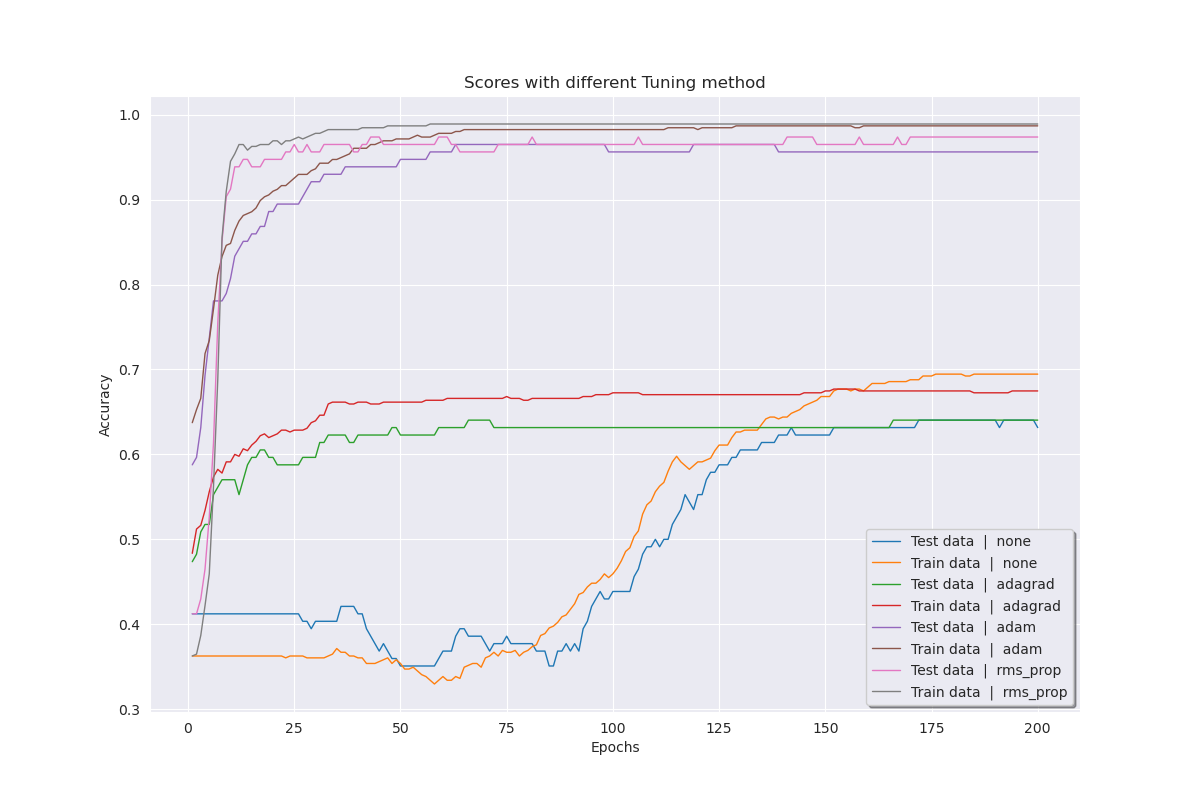
\includegraphics[width=0.8\textwidth]{Figures/PartD/d_tuning_eta_0_001_with_gamma_0.png}
    \caption{Accuracy score for test and data with different tuning methods
    plotted as function of epochs. Momentum ($\gamma $) is set to 0.}  
    \label{fig:d_tuning_eta_0_001_with_gamma_0_9} 
\end{figure}


\begin{figure}[H]
    \centering
    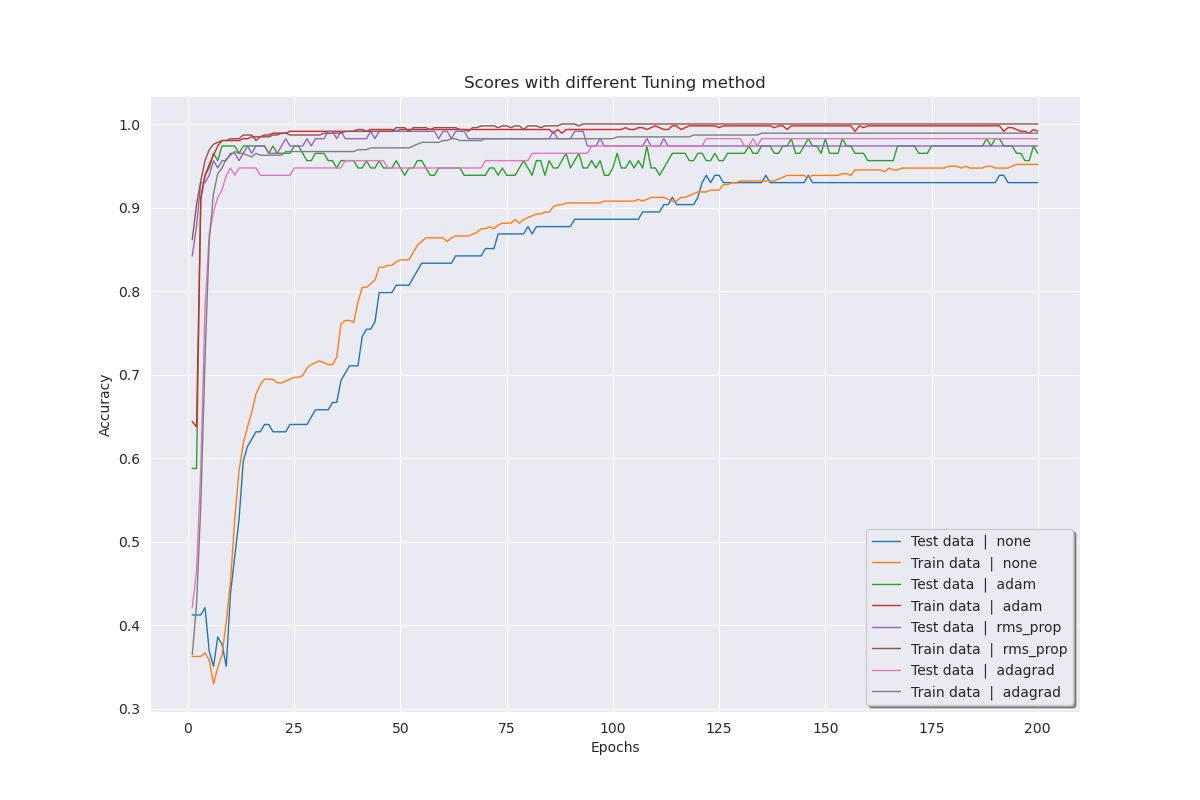
\includegraphics[width=0.8\textwidth]{Figures/PartD/d_tuning_eta_0_001_with_gamma_0_9.png}
    \caption{Accuracy score for test and data with different tuning methods
    plotted as function of epochs. Momentum ($\gamma $) is set to 0.9.}  
    \label{fig:d_tuning_eta_0_001_with_gamma_0_9} 

\end{figure}

%%%%%%%%%%%%%%% Run 5 %%%%%%%%%%%%%%%
% Activation function on hidden layers 

In run 5 we tested different activation functions on the hidden. From run 4 we
observed that both tuning method and added momentum improved the results
significantly. To understand better the different activation functions affect
the results we used a momentum parameter $\gamma = 0$ with constant learning
rate, $\eta = 0.001$. In figure \ref{fig:d_line_activation_hidden_gamma_0} the
accuracy is plotted for different activation functions in the hidden layers.
Both RELU and leaky RELU outperforms the sigmoid activation function. RELU and
Leaky RELU performs similar on the training data, but RELU gives the best
overall accuracy on the test data. 


\begin{figure}[H]
    \centering
    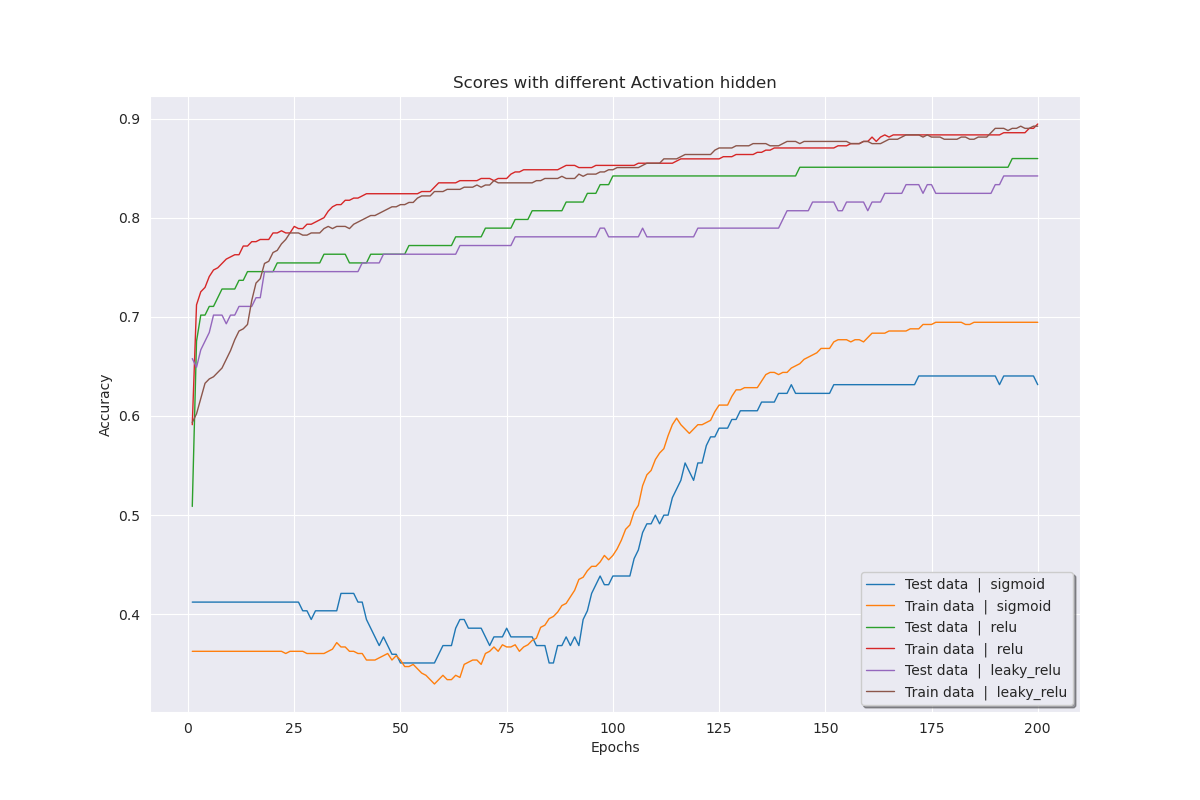
\includegraphics[width=0.8\textwidth]{Figures/PartD/d_line_activation_hidden_gamma_0.png}
    \caption{Accuracy score for train and test data with respect to epochs.
    Different activation functions on the hidden layers was used as indicated
in the label}  
\label{fig:d_line_activation_hidden_gamma_0} 
\end{figure}


%%%%%%%%%%%%%%% Run 6 %%%%%%%%%%%%%%%
% Combine best parameters









